% Original photograph, cropped only at display time. Labels remain editable.
% Crop rectangle in original pixels: (260,700)--(2850,3900), 72 dpi.
\begin{tikzpicture}
    \node[anchor=south west,inner sep=0] (photo) at (0,0)
        {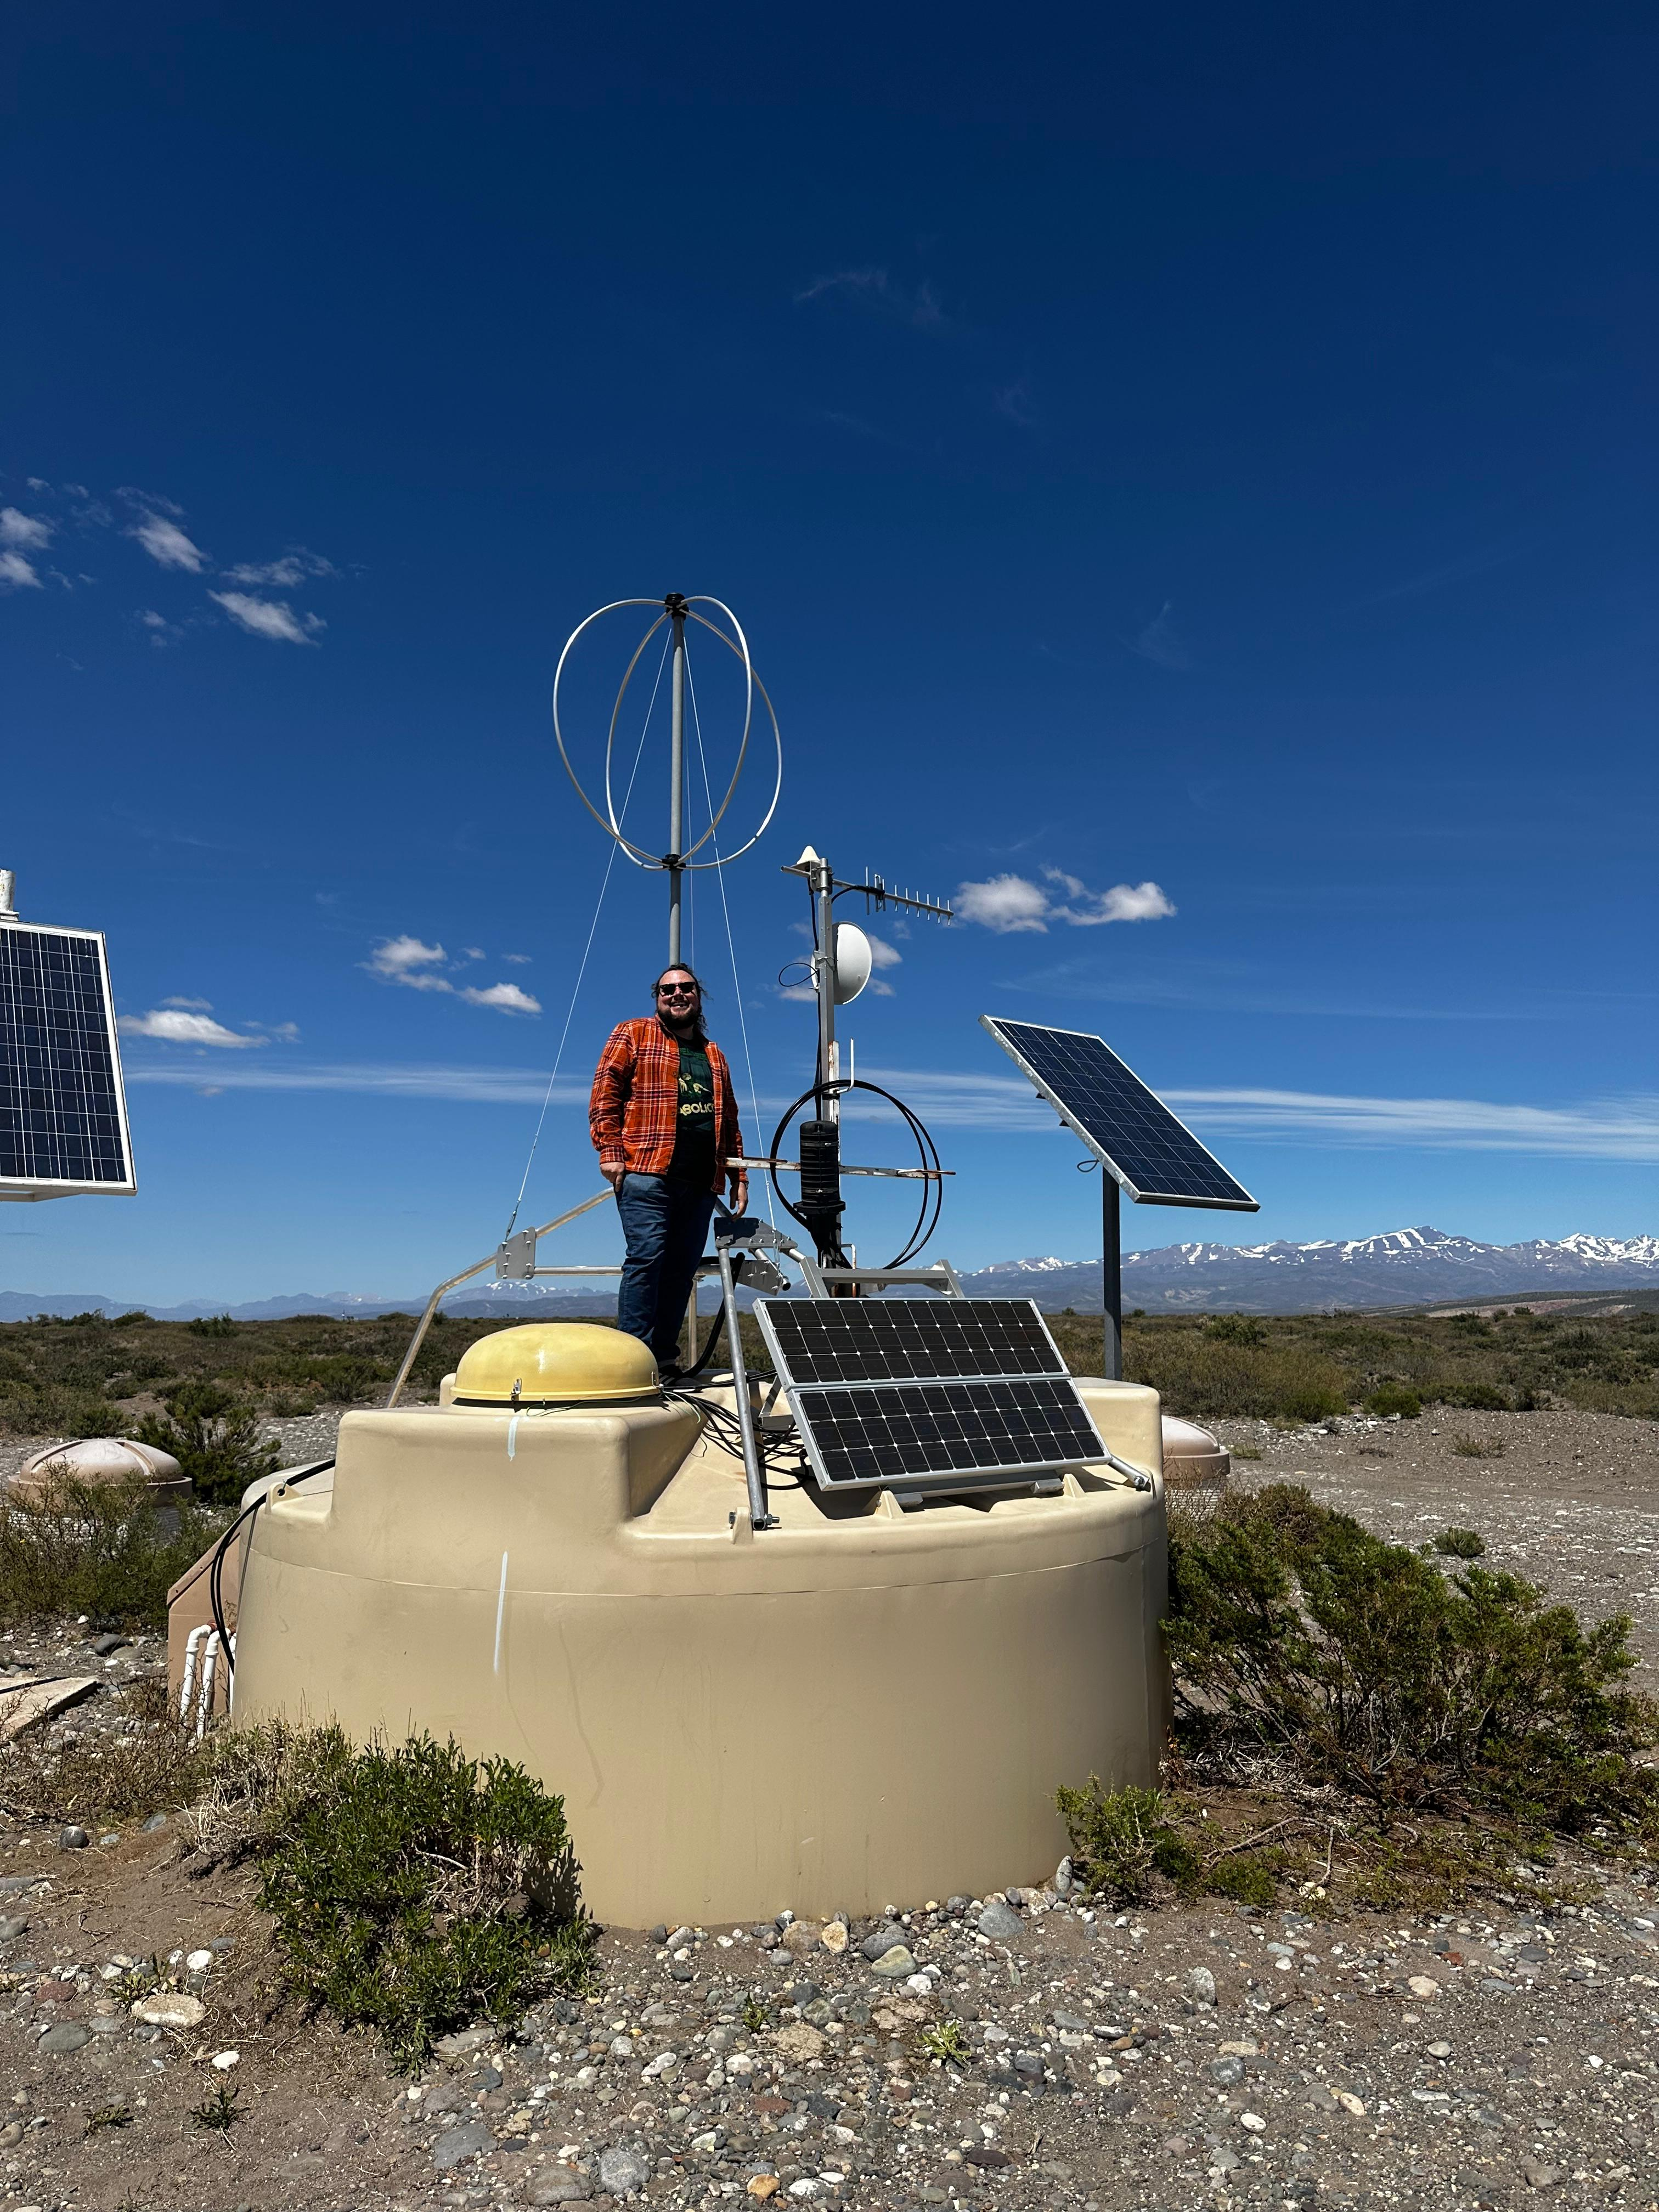
\includegraphics[width=\linewidth,trim=260bp 132bp 174bp 700bp,clip]{figures/chapter_auger/auger_station_reference.jpeg}};
    \begin{scope}[x={(photo.south east)},y={(photo.north west)}]
        \tikzset{component/.style={fill=white,draw=black,inner sep=2pt,align=center,font=\sffamily\scriptsize},
                 pointer/.style={->,>=stealth,line width=0.65pt,draw=yellow,preaction={draw=black,line width=1.15pt}}}
        \node[component] (gps) at (0.68,0.86) {GPS antenna};
        \draw[pointer] (gps.south west) -- (0.469,0.731);
        \node[component] (communication) at (0.79,0.74) {Communications\\antenna};
        \draw[pointer] (communication.west) -- (0.540,0.706);
        \node[component] (electronics) at (0.17,0.59) {Electronics\\box};
        \draw[pointer] (electronics.south) -- (0.286,0.441);
        \node[component] (solar) at (0.76,0.29) {Solar panel};
        \draw[pointer] (solar.north west) -- (0.544,0.413);
        \node[component] (battery) at (0.15,0.24) {Battery box};
        \draw[pointer] (battery.north west) -- (0.031,0.319);
    \end{scope}
\end{tikzpicture}
